\documentclass[12pt, a4paper]{extarticle}


% Russian text support
\usepackage[T2A]{fontenc}
\usepackage[utf8]{inputenc}
\usepackage[russian]{babel}

% Some useful packages
\usepackage{indentfirst}
\usepackage{etoolbox}
\usepackage{amsmath}
\usepackage{amssymb}
\usepackage{amsfonts}
\usepackage{xcolor}

% Pictures support
\usepackage{graphicx}
\graphicspath{ {../images/} }

% Page geometry
\usepackage[
    left=3cm,
    right=1cm,
    top=2cm,
    bottom=2cm
]{geometry}

% Make titles not to have numbering
\newenvironment*{dummyenv}{}{}

\newcommand{\mysection}[1]{
    \addcontentsline{toc}{section}{#1}
    \begin{dummyenv}
        \bfseries\large #1
    \end{dummyenv}
}

\makeatletter
\patchcmd{\l@section}
  {\hfil}
  {\leaders\hbox{\normalfont$\m@th\mkern \@dotsep mu\hbox{.}\mkern \@dotsep mu$}\hfill}
  {}{}
\makeatother

% Here we go...
\title{БДЗ по прикладной криптографии}
\author{Фирсов Георгий, М21-507}

\begin{document}

\maketitle

\tableofcontents

\pagebreak

\mysection{Задание 1}

Анна генерирует два числа $x \xleftarrow{R} \mathbb{Z}_1, y \xleftarrow{R} \mathbb{Z}_q$, после чего 
отсылает Борису тройку $(A_0, A_1, A_2) = (g^x, g^y, g^{xy + a})$.

Борис генерирует свои два числа $r \xleftarrow{R} \mathbb{Z}_q, s \xleftarrow{R} \mathbb{Z}_q$, а 
затем отправляет Анне следующую пару: $(B_1, B_2) = (A_1^r \cdot g^s, (A_2/g^b)^r \cdot A_0^s)$. 
Заметим, что:
\begin{equation*}
    \begin{split}
        & B_1 = A_1^r \cdot g^s = g^y \cdot g^s = g^{\textcolor{red}{y + s}} \\
        & B_2 = (A_2/g^b)^r \cdot A_0^s) = g^{xy + a} \cdot g^{-b} \cdot g^{xs} = 
        	g^{x(\textcolor{red}{y + s}) + a - b}
    \end{split}  
\end{equation*}

Если $B_1$ возвести в степень $x$ и затем умножить на обратный к полученному элемент число $B_2$, 
то получится $g^{a - b}$:
\begin{equation*}
    \begin{split}
        & B_1 ^ x = \left(g^{y + s}\right) ^ x = g^{x(y + s)} \\
        & B_2 \cdot (B_1^{-x}) = g^{x(y + s) + a - b} \cdot g^{-x(y + s)} = g^{a - b}
    \end{split}
\end{equation*}

Если $a = b$, то $g^{a - b} = g^0 = e_{\mathbb{G}}$. Это свойство и можно использовать для проверки 
равенства чисел $a$ и $b$.

\textbf{Ответ:} в) Анна проверяет равенство $B_2 / B_1^x = 1$.
\\

\mysection{Задание 2}

Так как числа $p, a, b$ общеизвестны, то считаю, что при разработке программы все \textit{возможные} 
вычисления с данными  параметрами выполняются заранее (то есть, собственно, на этапе разработки 
программы). Несложно увидеть, что:
\begin{equation*}
    \begin{split}
        H^{(n)}(x) & = \underbrace{H_{p,a,b}(H_{p,a,b}(\cdots H_{p,a,b}(x) \cdots))}_{\text{n раз}} = 
            \underbrace{a(a(\cdots\ ax + b\ \cdots) + b) + b}_{\text{n раз}} = \\
        & = a^n x + b \sum_{j=0}^{n - 1} a^j \mod p
    \end{split}
\end{equation*}

Обозначим:
\begin{equation*}
    \begin{split}
        & a' := a^n \mod p \\
        & b' := b \sum_{j=0}^{n - 1} a^j \mod p
    \end{split}
\end{equation*}

Тогда:
\begin{equation*}
    H^{(n)}(x) = a'x + b' \mod p
\end{equation*}

Значения $a'$ и $b'$ возможно вычислить предварительно на этапе разработки программы, что позволит 
вычислять функцию $H^{(n)}$ так же быстро, как и $H_{p,a,b}$.

Но может случиться так, что числа $p,a,b$ \textit{заранее} не известны (например, меняются с 
течением времени). Таким образом, возникает потребность поддержки вычисления $a', b'$ на лету. В 
таком случае заметим, что:
\begin{equation*}
    \begin{split}
        \sum_{j=0}^{n-1}a^j = (a^{n-1} - 1) \cdot (a - 1)^{-1} \mod p
    \end{split}
\end{equation*}

При больших $n$ возведение в степень $n-1$ потребует примерно столько же операций, сколько и 
возведение в степень $n$. Заметим, что возведение в степень можно производить, пользуясь следующей 
идеей: $a^4 = a^2 \cdot a^2, a^8 = a^4 \cdot a^4$ и т.д. Данный алгоритм требует асимптотически 
$\log _2(n)$ умножений.

\textbf{Ответ:} а) $H^{(n)}$ может быть вычислена так же быстро, как $H_{p,a,b}$ (в случае известных 
заранее значений $p,a,b$); г) вычисление $H^{(n)}$ требует времени $O(\log n)$ (в случае неизвестных 
заранее значений $p,a,b$).
\\

\mysection{Задание 3}

Рассмотрим по очереди все варианты, отобрав подходящие:
\begin{itemize}
    \item $p_1 = (k_1, k_2), p_2 = (k_1'), p_3 = (k_2')$: владельцы долей $p_2, p_3$ не смогут 
    	вдвоем восстановить ключ, так как $k_1' \oplus k_2' =\ ???$.
    
    \item $p_1 = (k_1, k_2), p_2 = (k_2, k_2'), p_3 = (k_2')$: владелец $p_2$ может один 
    	восстановить ключ, так как $k = k_2 \oplus k_2'$.
    
    \item $p_1 = (k_1, k_2), p_2 = (k_1, k_2), p_3 = (k_2')$: владельцы $p_1, p_2$ не смогут 
    	восстановить вдвоем ключ, так как никакая комбинация $k_1, k_2$ в сумме не даст $k$.
    
    \item $p_1 = (k_1, k_2), p_2 = (k_1', k_2'), p_3 = (k_2')$: владельцы $p_2, p_3$ не смогут 
    	восстановить вдвоем ключ, так как никакая комбинация $k_1', k_2'$ в сумме не даст $k$.
        
    \item $p_1 = (k_1, k_2), p_2 = (k_2'), p_3 = (k_1', k_2)$: данный вариант подходит, так как:
        \begin{itemize}
            \item $p_1, p_2$: $k_2  \oplus k_2' = k$
            \item $p_1, p_3$: $k_1  \oplus k_1' = k$
            \item $p_2, p_3$: $k_2' \oplus k_2  = k$
        \end{itemize}
        При этом восстановление ключа ни одним участником единолично невозможно, так как ни один 
        из них не обладает двумя частями с одинаковыми индексами.
\end{itemize}
\textbf{Ответ:} д) $p_1 = (k_1, k_2), p_2 = (k_2'), p_3 = (k_1', k_2)$
\\

\mysection{Задание 4}

Уязвимость протокола заключена в следующей фразе: ``Если все сертификаты и подписи проходят проверку 
с положительным результатом, то Анна считает, что она взаимодействует с Банком, и Банк считает, что 
он взаимодействует с Анной''.

Евгению достаточно иметь валидный сертификат и выработать валидную подпись, что верно в вариантах
ответа б и г. При этом он деперсонифицирует Анну и Банк соответственно.

В варианте б: сертификат является валидным сертификатом открытого ключа Евгения, подпись будет проверена
так же успешно. При этом Банк будет думать, что общается с Анной, хотя на самом деле общается с Евгением.

В варианте г: сертификат является валидным сертификатом открытого ключа Евгения, подпись будет проверена
так же успешно. При этом Анна будет думать, что общается с Банком, хотя на самом деле общается с Евгением.

Варианты а и в не позволяют Евгению получить общий с другой стороной ключ.

\textbf{Ответ:} б, г.
\\

\mysection{Задание 5}

\begin{enumerate}
    \item Так как каждому участнику $B_i, i \in \{1, ..., n\}$ известен ключ $k$, то, например, 
    	$B_2$ может создать некоторое сообщение и рассчитать имитовставку для него с использованием 
    	этого ключа. В таком случае участник $B_1$, получив сообщение, не может удостовериться, что 
    	оно создано участником $A$, а не $B_2$.
        
    \item При условии, что участники $B_i, i \in \{1, ..., n\}$ не вступают друг с другом в сговор, 
    	атака из п. 1 становится неприменимой, если:
        \begin{equation}
            \forall i,j \in \{1,...,n\} : i \ne j \implies S_i \setminus S_j \ne \varnothing
            \label{6.2-condition}
        \end{equation}
        
        Данное условие позволяет каждому участнику $B_i$ иметь хотя бы один такой ключ $k_m$, 
        которого нет у некоторого другого участника $B_j, j \ne i$. Такой ключ найдется у каждого 
        $B_i$ для каждого $B_j$. Таким образом, вероятность того, что подделанная имитовставка для 
        данного ключа окажется верной, является пренебрежимо малой при условии, что метод расчета 
        имитовставки является стойким.
        
        В то же время участник $A$ имеет все ключи и может рассчитать все имитовставки корректно.
        
    \item В таблице \ref{key-subsets} с помощью знака $+$ обозначено вхождение ключа 
    	$k_j, j \in \{1, ..., 5\}$ в подмножество $S_i, i \in \{1, ..., 10\}$, а знак $-$ обозначает 
    	отсутствие ключа в подмножестве.
        
        \begin{table}
            \caption{Состав подмножеств $S_j, j \in \{1, ..., 10\}$}
            \label{key-subsets}
            \centering
            \begin{tabular}{|c|c|c|c|c|c|}
                \hline
                Подмножество & $k_1$ & $k_2$ & $k_3$ & $k_4$ & $k_5$ \\
                \hline
                $S_1$    & $+$ & $+$ & $+$ & $-$ & $-$ \\
                \hline
                $S_2$    & $+$ & $+$ & $-$ & $+$ & $-$ \\
                \hline
                $S_3$    & $+$ & $+$ & $-$ & $-$ & $+$ \\
                \hline
                $S_4$    & $+$ & $-$ & $+$ & $+$ & $-$ \\
                \hline
                $S_5$    & $+$ & $-$ & $-$ & $+$ & $+$ \\
                \hline
                $S_6$    & $+$ & $-$ & $+$ & $-$ & $+$ \\
                \hline
                $S_7$    & $-$ & $+$ & $+$ & $+$ & $-$ \\
                \hline
                $S_8$    & $-$ & $+$ & $+$ & $-$ & $+$ \\
                \hline
                $S_9$    & $-$ & $+$ & $-$ & $+$ & $+$ \\
                \hline
                $S_{10}$ & $-$ & $-$ & $+$ & $+$ & $+$ \\
                \hline
            \end{tabular}
        \end{table}
        
        Несложно заметить, что любые попарные разности являются непустыми, так как все подмножества 
        имеют одинаковую мощность, равную трем, и попарно различны. Таким образом, условие 
        (\ref{6.2-condition}) выполнено, что обозначает неприменимость атаки из п. 1 к данной системе 
        (см. п. 2).
        
    \item Пусть в сговор вступают, например, $B_1$ и $B_9$. Заметим, что эти два участника вместе 
    	имеют в наличии все ключи $k_1, ..., k_5$. Если они обменяются недостающими ключами, то 
    	каждый из них может в таком случае рассчитать имитовставку для произвольного сообщения на 
    	каждом ключе и тем самым какой-либо другой участник не может быть уверен в том, что
        сообщение пришло от $A$, а не от $B_1$ или $B_9$.
\end{enumerate}

\mysection{Задание 6}

Анне и Борису известны следующий величины:
\begin{itemize}
    \item $v$
    \item $u = g^{\alpha} v^{-i}$
    \item Набор $u_j = u v^j = g^{\alpha} v^{j - i}, j \in \{1, ..., n\}$
\end{itemize}

Только Борису известны $\alpha$ и индекс $i$. Заметим, что для $j = i$: $u_i = g^{\alpha}$.

Анна пересылает Борису следующие значения:
\begin{equation*}
    (a_j, b_j) = \left(g^{k_j}, m_j u_j^{k_j}\right), k_j \xleftarrow{R} \{1, 2, ..., q-1\}
\end{equation*}

\begin{enumerate}
    \item \textit{Восстановление сообщения $m_i$ из полученных данных}.
        Борис может расшифровать значение $m_i$ (так как $\alpha$ -- закрытый ключ криптосистемы 
        Эль-Гамаля, соответствующий открытому ключу $u_i$):
        \begin{equation*}
            b_i a_i^{-\alpha} = m_i g^{\alpha k_i} g^{-k_i \alpha} = m_i
        \end{equation*}
        
    \item \textit{Невозможность получения индекса $i$ Анной}. Попробовать получить значение $i$ Анна 
    	может из значений $u = g^{\alpha} v^{-i}$ и $u_j = g^{\alpha} v^{j-i}$. Так как $v \in 
    	\mathbb{G}$, то $v = g^{k}$ для некоторого $k$. $u = g^{\alpha - ki}, u_j = g^{\alpha + 
    	k(j - i)}$.
        
        Заметим, что Анне неизвестны значения $\alpha, g^{\alpha}$. Отличить $u_i = g^{\alpha}$ 
        (даже если бы он был известен) от какого-то иного элемента группы вычислительно сложно, то 
        есть перебирая $j$ невозможно понять, когда $u_j$ сравняется с $g^{\alpha}$ (то есть при 
        $j = i$).
        
        Получить же $i$ из значения $u$ также вычислительно трудно, так как это предполагает 
        нахождение дискретного логарифма (по $u = g^{\alpha - ki}$ найти $\alpha - ki$ трудно).
\end{enumerate}

\mysection{Задание 7}

Преобразуем $\mathcal{F}$:
\begin{equation*}
    \begin{split}
        \mathcal{F}(x_1, x_2, x_3) & = (-5x_1^2+5x_1x_2+x_1x_3 - x_2x_3, 
            -3x_1+3x_1x_2+x_1x_3+3x_2-3x_2^2-x_2x_3) = \\
        & = \left((x_3 - 5x_1)(x_1 - x_2), (3x_2 + x_3 - 3)(x_1 - x_2)\right)
    \end{split}
\end{equation*}

Арифметическая схема для $\mathcal{F}$ изображена на рисунке \ref{arithmetic-circuit}.

\begin{figure}[h]
    \centering
    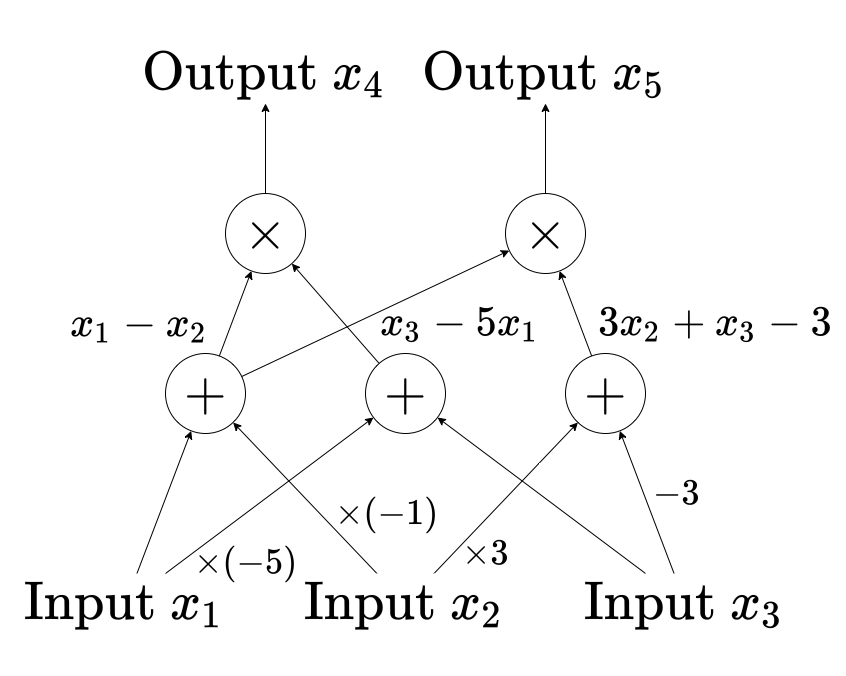
\includegraphics[width=0.7\textwidth]{arithmetic-circuit-hw_7.png}
    \caption{Арифметическая схема}
    \label{arithmetic-circuit}
\end{figure}

Построим по данной схеме квадратичную арифметическую программу:

\begin{enumerate}
    \item Построим множества $M, W$ и $I_{g, L}, I_{g, R}, g \in M$:
        \begin{equation*}
            \begin{split}
                & M = \{g_4, g_5\} \\
                & W = \{x_1, x_2, x_3, x_4, x_5\} \\
                & I_{g_4, L} = \{x_1, x_2\}, I_{g_4, R} = \{x_1, x_3\} \\
                & I_{g_5, L} = \{x_1, x_2\}, I_{g_5, R} = \{x_2, x_3\}
            \end{split}
        \end{equation*}
        
    \item Полином: $Z(z) = (z - r_4)(z - r_5)$, где $r_i \sim g_i, i \in \{4, 5\}$.
    
    \item Посчитаем значения полиномов $A_i(z)$ и $B_i(z), i \in \{0, ..., 5\}$ на корнях $Z(z)$.
        Значения представлены в табл. \ref{ab-values}.
        
        \begin{table}[h]
            \centering
            \caption{Значения полиномов $A_i(z), B_i(z), i \in \{0, ..., 5\}$ на корнях $Z(z)$}
            \label{ab-values}
            \begin{tabular}{|c|c|c|c|c|c|}
                \hline
                $A_0(r_4)$ & $A_1(r_4)$ & $A_2(r_4)$ & $A_3(r_4)$ & $A_4(r_4)$ & $A_5(r_4)$ \\
                \hline 
                0 & 1 & -1 & 0 & 0 & 0 \\
                \hline 
                $A_0(r_5)$ & $A_1(r_5)$ & $A_2(r_5)$ & $A_3(r_5)$ & $A_4(r_5)$ & $A_5(r_5)$ \\
                \hline 
                0 & 1 & -1 & 0 & 0 & 0 \\
                \hline 
                $B_0(r_4)$ & $B_1(r_4)$ & $B_2(r_4)$ & $B_3(r_4)$ & $B_4(r_4)$ & $B_5(r_4)$ \\
                \hline 
                0  & -5 & 0 & 1 & 0 & 0 \\
                \hline 
                $B_0(r_5)$ & $B_1(r_5)$ & $B_2(r_5)$ & $B_3(r_5)$ & $B_4(r_5)$ & $B_5(r_5)$ \\
                \hline 
                -3 & 0  & 3 & 1 & 0 & 0 \\
                \hline 
            \end{tabular}
        \end{table}
    
    \item Значения полиномов $C_i(z), i \in \{0, ..., 5\}$ на корнях $Z(z)$ приведены в табл. \ref{c-values}.
    
        \begin{table}[h]
            \centering
            \caption{Значения полиномов $C_i(z), i \in \{0, ..., 5\}$ на корнях $Z(z)$}
            \label{c-values}
            \begin{tabular}{|c|c|c|c|c|c|}
                \hline
                $C_0(r_4)$ & $C_1(r_4)$ & $C_2(r_4)$ & $C_3(r_4)$ & $C_4(r_4)$ & $C_5(r_4)$ \\
                \hline 
                0 & 0 & 0 & 0 & 1 & 0 \\
                \hline 
                $C_0(r_5)$ & $C_1(r_5)$ & $C_2(r_5)$ & $C_3(r_5)$ & $C_4(r_5)$ & $C_5(r_5)$ \\
                \hline 
                0 & 0 & 0 & 0 & 0 & 1 \\
                \hline 
            \end{tabular}
        \end{table}
        
    \item Получаются вот такие полиномы:
        \begin{equation*}
            \begin{split}
                & A_0(z) = A_3(z) = A_4(z) = A_5(z) \equiv 0 \\
                & A_1(z) = \frac{z - r_4}{r_5 - r_4} + \frac{z - r_5}{r_4 - r_5} \\
                & A_2(z) = \frac{z - r_4}{r_4 - r_5} + \frac{z - r_5}{r_5 - r_4} \\
                & B_4(z) = B_5(z) \equiv 0 \\
                & B_0(z) = 3 \cdot \frac{z - r_4}{r_4 - r_5} \\
                & B_1(z) = 5 \cdot \frac{z - r_5}{r_5 - r_4} \\
                & B_2(z) = 3 \cdot \frac{z - r_4}{r_5 - r_4} \\
                & B_3(z) = \frac{z - r_4}{r_5 - r_4} + \frac{z - r_5}{r_4 - r_5}
            \end{split}
        \end{equation*}
        
    \item В таком случае, получаем следующие $A, B$ и $C$:
        \begin{equation*}
            \begin{split}
                & A(z) = x_1 \cdot A_1(z) + x_2 \cdot A_2(z) \\
                & B(z) = B_0(z) + x_1 \cdot B_1(z) + x_2 \cdot B_2(z) + x_3 \cdot B_3(z) \\
                & C(z) = x_4 \cdot C_4(z) + x_5 \cdot C_5(z)
            \end{split}
        \end{equation*}
        
        Рассмотрим значения $P(z) = A(z) \cdot B(z) - C(z)$ на корнях $Z(z)$:
        \begin{equation*}
            \begin{split}
                P(r_4) & = A(r_4) \cdot B(r_4) - C(r_4) = \\
                & = \left(x_1 \cdot A_1(r_4) + x_2 \cdot A_2(r_4)\right)
                    \left(B_0(r_4) + x_1 \cdot B_1(r_4) + x_2 \cdot B_2(r_4) 
                    + x_3 \cdot B_3(r_4)\right) - x_4 = \\
                & = (x_1 - x_2)(x_3 - 5x_1) - x_4
            \end{split}
        \end{equation*}
        
        \begin{equation*}
            \begin{split}
                P(r_5) & = A(r_5) \cdot B(r_5) - C(r_5) = \\
                & = \left(x_1 \cdot A_1(r_5) + x_2 \cdot A_2(r_5)\right)
                    \left(B_0(r_5) + x_1 \cdot B_1(r_5) + x_2 \cdot B_2(r_5) 
                    + x_3 \cdot B_3(r_5)\right) - x_5 = \\
                & = (x_1 - x_2)(3x_2 + x_3 - 3) - x_5
            \end{split}
        \end{equation*}
        
        Таким образом, $Z(z) | P(z)$ $\iff$ $r_4, r_5$ являются корнями $P(z)$, т.е. 
        $(x_1, x_2, x_3, x_4, x_5)$ -- корректное назначение для исходной арифметической схемы.
        
        Требуемая квадратичная арифметическая программа -- $Q(C) = \left(\vec{A}, \vec{B}, \vec{C}, 
        Z \right)$
\end{enumerate}

\mysection{Задание 8}

Для расшифрования сообщения, зашифрованного на ключе $g^{\alpha}$, используется следующий алгоритм:
\begin{equation*}
    \begin{split}
        & k \leftarrow H\left(v^{\alpha}\right) = H\left(g^{\beta \alpha}\right) \\
        & m \leftarrow E_k^{-1}(c)
    \end{split}
\end{equation*}

\begin{enumerate}
    \item \textit{Использование величины} $\tau$. Сервер транслирует сообщения, зашифрованные на ключе
        $g^{\alpha}$, в зашифрованные на ключе $g^{\alpha'}$ путем следующей процедуры:
        \begin{equation*}
            (v', c') = (v^{\tau}, c)
        \end{equation*}
        
        Проверим, что теперь расшифровать сообщение можно при помощи закрытого ключа $\alpha'$:
        \begin{equation*}
            \begin{split}
                & k \leftarrow \textcolor{red}{H(g^{\beta \alpha})} \\
                & k \leftarrow H({v'}^{\alpha'}) = H(v^{\tau \alpha'}) = H(v^{\frac{\alpha 
                    \alpha'}{\alpha'}}) = H(v^{\alpha}) = \textcolor{red}{H(g^{\beta \alpha})}
            \end{split}
        \end{equation*}
        
        Первое выражение для $k$ -- оригинальное значение, использовавшееся при первоначальном
        зашифровании на ключе $g^{\alpha}$. Второе выражение -- значение ключа, получаемое Анной
        при расшифровании. Несложно заметить, что они равны, а значит теперь Анна может
        расшифровать сообщение.
        
    \item \textit{Трансляция в обратном направлении}. Используется все тот же алгоритм из п. 1,
        но $v$ возводится в степень $\tau^{-1}$.
        
    \item \textit{Прекращение возможности трансляции}. Борису достаточно сменить ключевую пару,
        так как в этом случае сообщения будут зашифровываться уже на другом симметричном ключе,
        вырабатываемом по схеме, указанной в задании, что сделает невозможным чтение их Анной,
        потому что значение $\tau$ уже не выражает связь ее закрытого ключа с ключом Бориса.
        
        Стоит отметить, что сменив ключи перед уходом в отпуск, Борис может быть уверенным, что
        Анна не сможет прочитать письма, пришедшие ему до ухода в отпуск (подразумевается, что
        для согласования значения $\tau$ используется новая ключевая пара).
\end{enumerate}

\mysection{Задание 9}

Так как $\text{ord }\mathbb{G} = q$ -- простое число, то все элементы группы, не равные 
$e_{\mathbb{G}}$, являются образующими. Это значит, что взяв случайный неединичный элемент группы, 
гарантированно можно получить образующий.

\begin{enumerate}
    \item Общеизвестными параметрами схемы мультикоммитмента являются: простое число $q$, группа 
    	$\mathbb{G}$ порядка $q$, а также случайные $(h, g_1, ..., g_n)$, для которых выполнено:
        \begin{equation*}
            \begin{split}
                & h \in \mathbb{G}, h \ne e_{\mathbb{G}} \\
                & \forall i \in \{1, ..., n\} : g_i \in \mathbb{G}, g_i \ne e_{\mathbb{G}} \\
                & \forall i, j \in \{1, ..., n\} : g_i \ne h; i \ne j \implies g_i \ne g_j
            \end{split}
        \end{equation*}
        
        Пусть $r \xleftarrow{R} \mathbb{Z}_q$. Функция $Commit_n$ выглядит следующим образом:
        \begin{equation}
            Commit_n(\mathbf{m}, r) = h^r \prod_{j = 1}^{n} g_j^{m_j}, \mathbf{m} = (m_1, ..., m_n)
            \label{9.1-multicommitment}
        \end{equation}
        
        Несложно показать свойство гомоморфизма:
        \begin{equation*}
            \begin{split}
                Commit_n(\mathbf{m} + \mathbf{m'}, &\ r + r') = h^{r + r'} \prod_{j = 1}^{n} 
                	g_j^{m_j + m'_j} = h^r h^{r'} \left(\prod_{j = 1}^{n} g_j^{m_j}\right) 
                	\left(\prod_{j = 1}^{n} g_j^{m'_j}\right) = \\
                & = \left(h^r \prod_{j = 1}^{n} g_j^{m_j}\right) \left(h^{r'} 
                	\prod_{j = 1}^{n} g_j^{m'_j}\right) = Commit_n(\mathbf{m}, r) +
                	Commit_n(\mathbf{m'}, r')
            \end{split}
        \end{equation*}
        
    \item Покажем, что схема, описанная в п. 1 обеспечивает совершенное сокрытие. Для этого следует 
    	показать, что для любых векторов $\mathbf{m} = (m_1, ..., m_n)$ и $\mathbf{m'} = (m'_1, ..., 
    	m'_n)$ равны распределения следующих случайных величин:
        \begin{equation*}
            \begin{split}
                & C  = Commit_n(\mathbf{m},  r),  r  \xleftarrow{R} \mathbb{Z}_q \\
                & C' = Commit_n(\mathbf{m'}, r'), r' \xleftarrow{R} \mathbb{Z}_q
            \end{split}
        \end{equation*}
        где $Commit_n$ определена согласно (\ref{9.1-multicommitment}).
        
        Обозначим через $\alpha_i, i \in \{1, ..., n\}$ такие числа, что $g_i^{\alpha_i} = h$ 
        (такое число всегда найдется, так как $g_i$ -- образующий элеемент группы $\mathbb{G}$). 
        Положим также:
        \begin{equation*}
            \alpha = \sum_{j = 1}^{n} \alpha_j m_j,\ \alpha' = \sum_{j = 1}^{n} \alpha_j m'_j
        \end{equation*}
        
        Пусть $r \xleftarrow{R} \mathbb{Z}_q$, тогда $c = Commit_n(\mathbf{m}, r) = h^{r + \alpha}$ 
        и $c' = Commit_n(\mathbf{m'}, r) = h^{r + \alpha'}$ ($c$ -- розыгрыш случайной величины $C$, 
        $c'$ -- величины $C'$).
        
        Из вычислительной сложности задачи дискретного логарифмирования следует, что $c$ и $c'$ 
        отличить друг от друга так же вычислительно сложно, из чего, в свою очередь, следует 
        равенство распределений случайных величин $C$ и $C'$.
        
    \item В п. 1 утверждалось, что $h, g_i, i \in \{1, ...,n\}$ -- случайные неединичные элементы 
        группы $\mathbb{G}$. Также в примечании перед п. 1 утверждается, что любой неединичный 
    	элемент из $\mathbb{G}$ является образующим. Упомянутые элементы группа можно получить 
    	следующим образом:
        \begin{equation}
            \begin{split}
                & h = H(i_1) \\
                & g_j = H(i_{j + 1}), j \in \{1, ..., n\}
            \end{split}
            \label{9.3-elems-generation}
        \end{equation}
        где $H:\mathbb{Z}_q \to \mathbb{G}$ -- случайный оракул, а последовательность 
        $\{i_j\}_{j=1}^{n+1}$ составляется следующим образом:
        \begin{equation*}
            \begin{split}
                & i_1 = k_0 \\
                & i_{j+1} = i_j + k_j
            \end{split}
        \end{equation*}
        где $k_0$ -- минимальное положительное число, при котором $H(k_0) \ne e_{\mathbb{G}}$, 
        $k_j$ -- минимальное положительное число, при котором $H(i_j + k_j) \ne e_{\mathbb{G}}$ и не 
        совпадает с предыдущими значениями.
        
        Таким образом, элементы, сгенерированные по формулам в (\ref{9.3-elems-generation}) являются 
        случайными образующими элементами группы $\mathbb{G}$, вероятность совпадений среди которых 
        мала. Т.е. они удовлетворяют требованиям из п. 1.
        
        Свойство сокрытия показано в п. 2. Свойство связывания следует из вычислительной сложности 
        задачи логарифмирования: из этого следует отсутствие эффективного алгоритма для генерации 
        таких $r, r', \mathbf{m}, \mathbf{m'}$, что $Commit_n(\mathbf{m}, r) = 
        Commit_n(\mathbf{m'}, r')$.
\end{enumerate}

\mysection{Задание 10}

\begin{enumerate}
    \item \textit{Некорректное хэширование}. Так как требуется подделка подписи для любого сообщения, 
    	то рассматривается модель стойкости UUF-CMA (Universal Unforgeability under Chosen Message 
    	Attack). Рассмотрим противника $\mathcal{A}$, действующего по следующему сценарию:
        \begin{itemize}
            \item $\mathcal{A}$ генерирует некоторое сообщение $m \in \mathcal{M}$ (любое).
            
            \item $\mathcal{A}$ вычисляет хэш сообщения: $c = H(m)$.
            
            \item $\mathcal{A}$ вычисляется значение $R = h^{-c}$ ($h = pk$), значение $z$ полагается 
            	равным 0.
            
            \item Подпись $\sigma = (R, z) = (pk^{-H(m)}, 0)$ отправляется оракулу проверки подписи.
        \end{itemize}
        
        Заметим, что проверка этой подписи выполнится всегда:
        \begin{equation*}
            \left.\begin{array}{l}
                c \leftarrow H(m) \\
                \textcolor{red}{g^z} = \textcolor{red}{e_{\mathbb{G}}} \\
                \textcolor{red}{R \cdot h^c} = h^{-H(m)} \cdot h^{H(m)} = h^0 = 
                    \textcolor{red}{e_{\mathbb{G}}}
            \end{array}\right\} \implies V(pk, m, \sigma) = \text{accept}
        \end{equation*}
        
        Таким образом:
        \begin{equation*}
            \textbf{Adv}_{\text{SS}}^{\text{UUF-CMA}}(\mathcal{A}) = 
                \text{Pr}[V(pk, m, \sigma) = \text{accept}] = 1
        \end{equation*}
        
    \item \textit{Некорректная генерация случайных чисел}. Обозначим $c_i = H(m_i, R_i), 
   		i \in \{0, 1\}$ и, зная, что $\rho_1 = a \rho_0 + b$, запишем:
        \begin{equation*}
            \begin{split}
                & \left\{\begin{array}{l}
                    z_0 = \rho_0 + c_0 \alpha \\
                    z_1 = a \rho_0 + b + c_1 \alpha
                \end{array}\right. \\ \\
                & \left\{\begin{array}{l}
                    a z_0 = a \rho_0 + a c_0 \alpha \\
                    z_1 = a \rho_0 + b + c_1 \alpha
                \end{array}\right.
            \end{split}
        \end{equation*}
        
        Тогда:
        \begin{equation*}
            \begin{split}
                & z_1 - a z_0 = b + \alpha (c_1 - a c_0) \\
                & \alpha = (z_1 - a z_0 - b)(c_1 - a c_0)^{-1}
            \end{split}
        \end{equation*}
        
        В общем-то $(c_1 - a c_0)$ -- некоторый случайный элемент из $\mathbb{Z}_q$, а так как 
        $q$ -- простое число, то для обратимости элемента требуется только то, чтобы он был 
        ненулевым. Вероятность того, что элемент $(c_1 - a c_0)$ обратим, равна:
        \begin{equation*}
            \text{Pr}\left[\begin{array}{c}
                \text{Элемент } (c_1 - a c_0) \\
                \text{обратим в кольце } \mathbb{Z}_q
            \end{array}\right] = 1 - \frac{1}{|\mathbb{Z}_q|} = \frac{q - 1}{q} 
            	\xrightarrow[q \to \infty]{} 1
        \end{equation*}
        
    \item \textit{Атака по взаимосвязанным ключам}. Пусть $pk_i = h \cdot g^i = g^{\alpha} 
    	\cdot g^i = g^{\alpha + i}$, тогда через обозначим $sk_i = \alpha_i = \alpha + i$ 
    	(согласно нотации криптосистемы). Введем также обозначение $\Delta\alpha_{ij} := j - i$.
        
        Пусть для некоторого сообщения $m$ имеется некоторая подпись $\sigma_i = (R_i, z_i)$, 
        где $z_i = \rho_i + c_i \alpha_i$, $c_i = H(m, R_i)$. Противник генерирует следующую подпись: 
        $\sigma_j = (R_i, z_j)$, где $z_j = \rho_i + c_i \alpha_i + c_i \Delta\alpha_{ij} = 
        \rho_i + c_i\alpha_j$. 
        
        Эта подпись является валидной для того же сообщения и успешно проверяется на ключе $pk_j$:
        \begin{equation*}
            \left.\begin{array}{l}
                c = H(m, R_i) \\
                g^{z_j} = g^{\rho_i + c_i\alpha_j} = \textcolor{red}{g^{\rho_i + c_i(\alpha + j)}} \\
                R_i \cdot pk_j^{c} = g^{\rho_i} \cdot g^{c(\alpha + j)} = 
                    \textcolor{red}{g^{\rho_i + c(\alpha + j)}}
            \end{array}\right\} \implies V(pk_j, m, \sigma_j) = \text{accept}
        \end{equation*}
\end{enumerate}

\mysection{Задание 11}

\begin{enumerate}
	\item Пусть пассивный противник записал успешный сеанс протокола аутентификации, то есть в его
		распоряжении находятся запрос $m$ и ответ $t$. при этом также известно, что $t = MAC(sk, m)$
		для некоторого $sk$, являющегося в данном случае паролем.
		
		Перебирая $sk$ по словарю и сравнивая получаемые значения имитовставки от $m$, рассчитанной
		на перебираемом значении в качестве ключа, с $t$, противник может найти подходящее значение
		$sk$. Ясно, что успешность атаки зависит от размера словаря и самого пароля, однако словарная
		атака на такую схему аутентификации в принципе возможна.
		
	\item Пусть активный противник как бы ``подменяет'' сервер и отдает клиенту свой сертификат
		$Cert_E$. Если клиент не проверяет сертификат должным образом, то он будет считать, что
		общается с сервером, хотя на самом деле обмен пакетами происходит с противником\footnote{
		Противник при этом может проксировать запросы на настоящий сервер для сокрытия своего
		присутствия. Это возможно, если он сам установит соединение с сервером.}.
		
		Сгенерировав запрос\footnote{Это не понадобится, если противник проксирует запросы/ответы 
		с/на сервер. Кроме того, такое проксирование позволит убедиться в правильности ответа
		клиента.} и получив ответ, противник получает в распоряжение пару $m, t$ запроса
		и ответа, которая может использоваться для проведения словарной атаки (см. п. 1). 
	
	\item Проведем некоторые преобразования:
		\begin{equation*}
			\begin{split}
				& U_2 = (S / h^{pw})^u = (g^s h^{pw} / h^{pw})^u = g^{su} \\
				& U_1 U_2 = g^u k^{pw} g^{su} = g^{u(s + 1)} k^{pw}
			\end{split}
		\end{equation*}
		
		Сервер получает $U_1 = g^u k^{pw}$ и $U_3 = H(pw, S, U_1 U_2)$. При этом серверу требуется
		рассчитать хэш от набора значений $pw, S, U_1 U_2$ и сравнить с полученным $U_3$. $S$ и 
		$pw$ серверу известны, надо посчитать значение $U_1 U_2$, что можно сделать следующим
		образом:
		\begin{equation*}
			U_1 U_2 = g^{u(s + 1)} k^{pw} = \frac{g^{u(s + 1)} k^{pw} k^{s \cdot pw}}{k^{s \cdot pw}} =
				\frac{g^{u(s + 1)} k^{pw \cdot (s + 1)}}{k^{s \cdot pw}} =
				\frac{(g^u k^{pw})^{s + 1}}{k^{s \cdot pw}} = 
				\frac{U_1^{s + 1}}{k^{s \cdot pw}}	
		\end{equation*}
		что возможно, так как $s$ и $k$ серверу так же известны.
		
		Таким образом, на сервере осуществляется проверка ниже, а сеанс аутентификации считается
		успешным, если она пройдена.
		\begin{equation*}
			U_3 \stackrel{?}{=} H\left(pw, S, \frac{U_1^{s + 1}}{k^{s \cdot pw}}\right)
		\end{equation*}
\end{enumerate}

\mysection{Задание 12}

:(

\end{document}
